\documentclass{tufte-handout}

%\geometry{showframe}% for debugging purposes -- displays the margins
\usepackage{amsmath}
\setcitestyle{authoryear,open={(},close={)}}
% Set up the images/graphics package
\usepackage{graphicx}
\setkeys{Gin}{width=\linewidth,totalheight=\textheight,keepaspectratio}
\graphicspath{{graphics/}}

\title{Activity 4: Classifying stellar spectra}
\author[Dr. N\'estor Espinoza]{Dr. N\'estor Espinoza}
\date{January, 2019}  % if the \date{} command is left out, the current date will be used

% The following package makes prettier tables.  We're all about the bling!
\usepackage{booktabs}

% The units package provides nice, non-stacked fractions and better spacing
% for units.
\usepackage{units}

% The fancyvrb package lets us customize the formatting of verbatim
% environments.  We use a slightly smaller font.
\usepackage{fancyvrb}
\fvset{fontsize=\normalsize}

% Small sections of multiple columns
\usepackage{multicol}

% Provides paragraphs of dummy text
\usepackage{lipsum}

% These commands are used to pretty-print LaTeX commands
\newcommand{\doccmd}[1]{\texttt{\textbackslash#1}}% command name -- adds backslash automatically
\newcommand{\docopt}[1]{\ensuremath{\langle}\textrm{\textit{#1}}\ensuremath{\rangle}}% optional command argument
\newcommand{\docarg}[1]{\textrm{\textit{#1}}}% (required) command argument
\newenvironment{docspec}{\begin{quote}\noindent}{\end{quote}}% command specification environment
\newcommand{\docenv}[1]{\textsf{#1}}% environment name
\newcommand{\docpkg}[1]{\texttt{#1}}% package name
\newcommand{\doccls}[1]{\texttt{#1}}% document class name
\newcommand{\docclsopt}[1]{\texttt{#1}}% document class option name


\titlespacing*{\section}{0pt}{0.3\baselineskip}{\baselineskip}
\begin{document}

\noindent\textcolor{Red}{\rule{16cm}{3mm}}

{\let\newpage\relax\maketitle}
%\maketitle% this prints the handout title, author, and date

\begin{abstract}
\noindent\textcolor{Red}{\rule{10cm}{0.4mm}}
\noindent In this activity, we will once again use spectra from the Sloan Digital Sky Survey (SDSS), but this time 
of many stars in order to find patterns that can help us clasify them. The activity aims at solidifying the analysis of 
the spectra of stars as well as the understanding of physical properties stellar spectra have in common, providing in turn 
hints to possible physical similarities between the objects.
\noindent\textcolor{Red}{\rule{10cm}{0.4mm}}
\end{abstract}


\section{Instructions}\label{sec:intro}
\begin{fullwidth}
The data we show in Figures \ref{fig:spectra}, \ref{fig:spectra2} and \ref{fig:spectra3} was taken from the Sloan Digital Sky Survey (SDSS) 
SkyServer\footnote{\url{http://skyserver.sdss.org}}. This is a server which hosts up-to-date data taken mainly from the 
2.5m SDSS Telescope in Apache Point, New Mexico. 

\textbf{Form groups of 5-6 people} and try to generate a classification scheme for the stellar spectra presented in Figures \ref{fig:spectra}, 
\ref{fig:spectra2} and \ref{fig:spectra3}. Select one or two persons from your group to present this classification scheme to the class in no 
more than 3 minutes, identifying patterns and particularities of the stellar spectra under your classification scheme. 
\textbf{Put a name to your classification scheme}.

\begin{figure}
  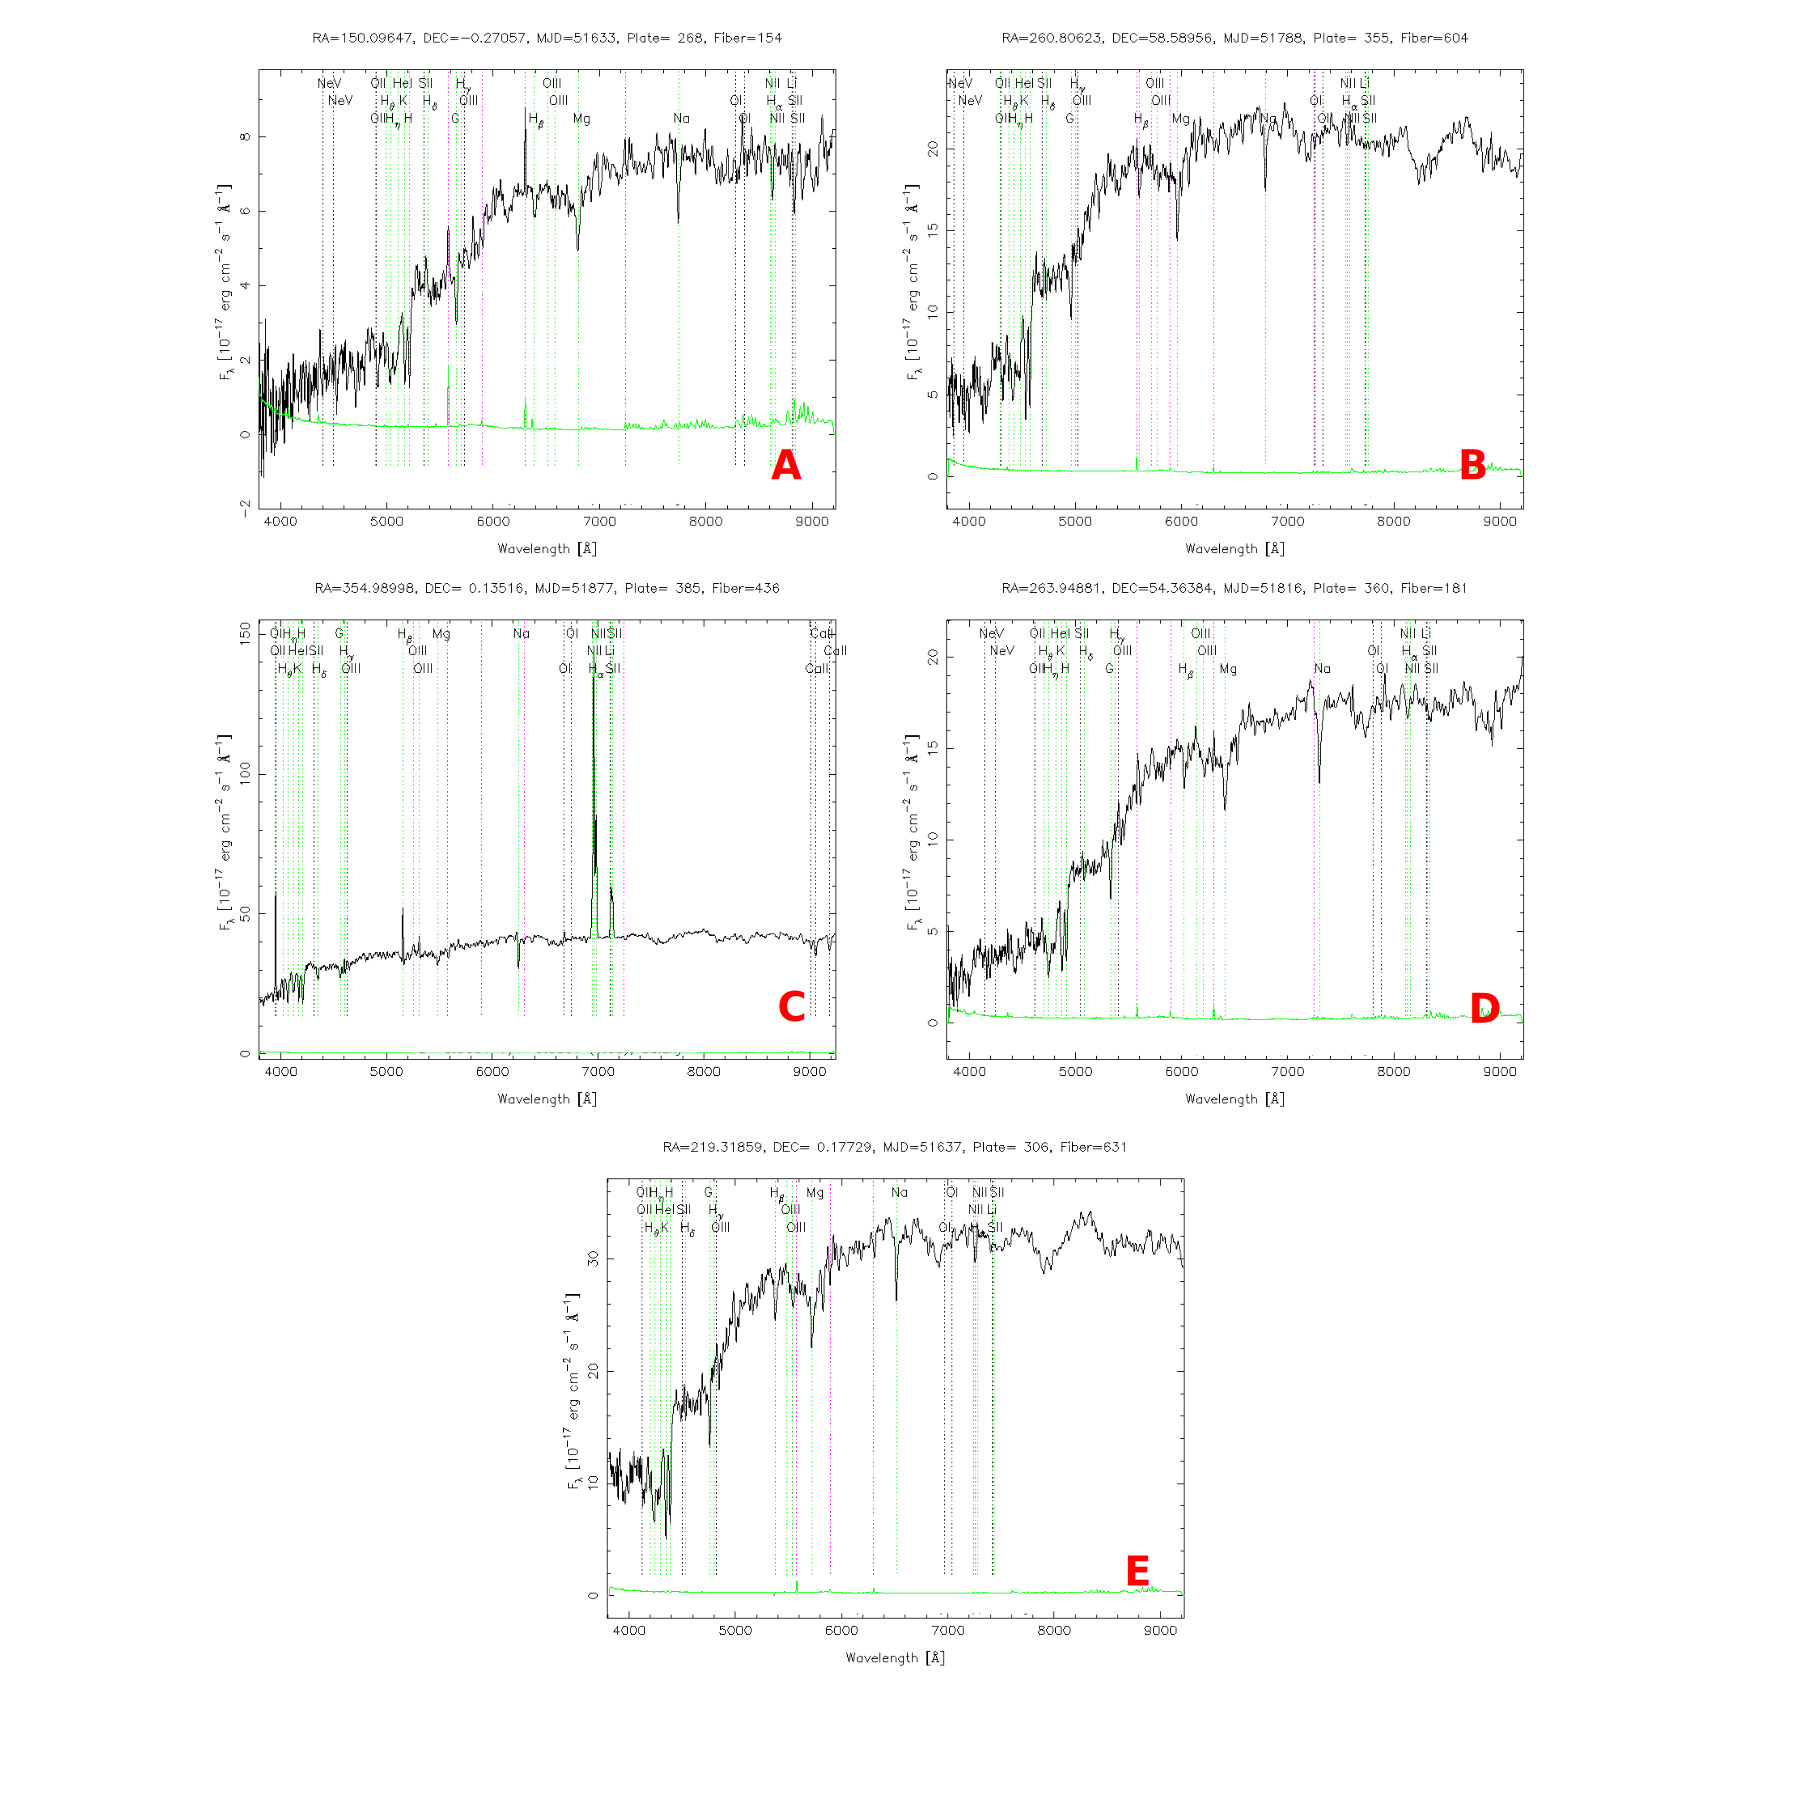
\includegraphics[width=2.0\columnwidth]{figures_activity4/spectra1.pdf}
%  \checkparity This is an \pageparity\ page.%
  \caption{Set of real star spectra for the activity. Data taken from the SDSS.}
  \label{fig:spectra}
  %\zsavepos{pos:textfig}
  \setfloatalignment{b}
\end{figure}

\begin{figure}
  \includegraphics[width=2.0\columnwidth]{figures_activity4/spectra2.pdf}
%  \checkparity This is an \pageparity\ page.%
  \caption{Set of real star spectra for the activity. Data taken from the SDSS.}
  \label{fig:spectra2}
  %\zsavepos{pos:textfig}
  \setfloatalignment{b}
\end{figure}

\begin{figure}
  \includegraphics[width=2.0\columnwidth]{figures_activity4/spectra3.pdf}
%  \checkparity This is an \pageparity\ page.%
  \caption{Set of real star spectra for the activity. Data taken from the SDSS.}
  \label{fig:spectra3}
  %\zsavepos{pos:textfig}
  \setfloatalignment{b}
\end{figure}

\end{fullwidth}

%\begin{enumerate}
%\item Introduction (day 1).
%\item Cosmology, pt. I (day 2).
%\item Cosmology, pt. II (day 3).
%\item Stellar formation and evolution (day 4).
%\item Exoplanets (day 5).
%\end{enumerate}
%We describe each of these units below.
%\end{fullwidth}
%\subsection{Headings}\label{sec:headings}

%\begin{table}[ht]
%  \centering
%  \fontfamily{ppl}\selectfont
%  \begin{tabular}{ll}
%    \toprule
%    Margin & Length \\
%    \midrule
%    Paper width & \unit[8\nicefrac{1}{2}]{inches} \\
%    Paper height & \unit[11]{inches} \\
%    Textblock width & \unit[6\nicefrac{1}{2}]{inches} \\
%    Textblock/sidenote gutter & \unit[\nicefrac{3}{8}]{inches} \\
%    Sidenote width & \unit[2]{inches} \\
%    \bottomrule
%  \end{tabular}
%  \caption{Here are the dimensions of the various margins used in the Tufte-handout class.}
%  \label{tab:normaltab}
%  %\zsavepos{pos:normaltab}
%\end{table}


\end{document}
